\documentclass[main.tex]{subfiles}

\begin{document}

\section*{Goal}
For our final experiment, we will investigate the wave properties of sound to determine the wavelength of a standing wave in a pipe.

\section*{Equipment}
\begin{itemize}
\item
Standing Wave Tube
\item
Tuning Forks
\item
Meter Stick
\end{itemize}•

\section*{Theory}
\begin{wrapfigure}[10]{r}{0.5\textwidth}
\centering
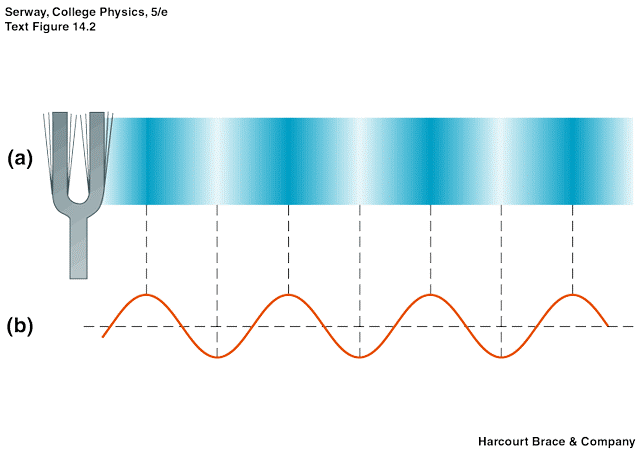
\includegraphics[width=0.5\textwidth]{Sound_longitudinal}
\caption{} \label{fig:Longitudinal}
\end{wrapfigure}
Sound can be described as a longitudinal wave where the molecules of the atmosphere vibrate back-and-forth, creating small oscillations in pressure that we interpret as sound. Like all pure, harmonic waves, we can describe a sound in terms of its wavelength $\lambda,$ its frequency $\nu,$ and its velocity $v.$ The wavelength is the minimum length (at one moment) of one complete cycle of the pressure, e.g., from maximum to maximum. The frequency is the number of cycles that occur in a given unit of time (at one fixed position). We can relate these quantities by,
\begin{equation} \label{eq:Waves}
v=\nu\lambda.
\end{equation}
Equation~\eqref{eq:Waves} is true for all waves, whether they be sound, light, mechanical, etc. However, since sound requires a medium to transmit through, the velocity of sound is dependent on the temperature of the medium. In air, the temperature dependence on $v$ is given by,
\begin{equation} \label{eq:Vsound}
v=331 \text{m}/\text{s} + 0.62 T,
\end{equation}
where $T$ is the temperature given in $\celsius$ and 331 m/s is the velocity of sound at $0\celsius.$

The phenomenon of resonance occurs when the natural frequency of vibration of a body is the same as the exciting frequency. In our experiment, the resonating body will be the column of air in a tube. When sound vibrations are fed into the tube, the waves travel down the tube and are reflected by the surface of water in the bottom of the tube. If the length of the column of air above the water is at an odd multiple of a quarter-wavelength, then the reflected waves will reinforce the incoming waves and the column of air will resonate. At resonance, the sound will increase in intensity and thus be louder.

\begin{wrapfigure}{R}{0.5\textwidth}
\centering
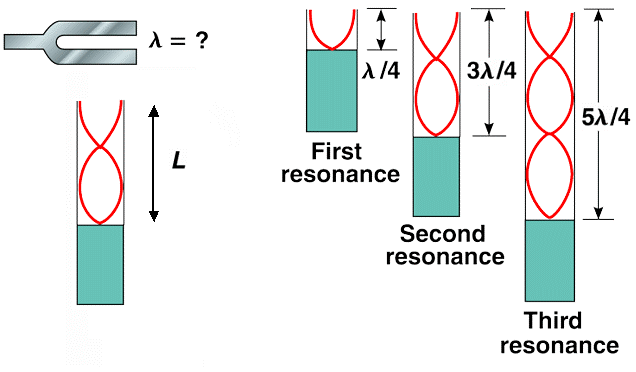
\includegraphics[width=0.5\textwidth]{Sound_Resonance}
\caption{} \label{fig:Resonance}
\end{wrapfigure}
The resonance occurs whenever there is a \emph{node}---where the wave has zero amplitude along its propagating axis---at the water and an \emph{antinode}---where the wave has maximum amplitude---at the opening of the tube. As we can see in Figure~\ref{fig:Resonance}, we let $L$ be the distance from the opening of the tube to the water level. For the first resonance, $L_1=\lambda/4$ or $\lambda=4L_1,$ the second resonance $L_2=3\lambda/4$ or $\lambda=4L_2/3,$ and so on. In general we can determine the $n$th resonance as,
\begin{equation} \label{eq:Resonance}
L_n=\frac{2n-1}{4}\lambda,
\end{equation}
or
\begin{equation} \label{eq:Wavelength}
\lambda=\frac{4}{2n-1}L_n.
\end{equation}•

\section*{Procedure}
\begin{enumerate}
\item \label{step:velocity}
Read the temperature in $\celsius$ from the wall-mounted thermometer in the back of the classroom. Use Equation~\eqref{eq:Vsound} to calculate the velocity of sound in the room.
\item
All lengths are measured from the mouth of the tube downwards. Mount the tuning fork about 1 cm from the mouth of the tube.
\item
Fill the reservoir until the water reaches 10 cm from the mouth of the tube.
\item
Using the frequency marked on the tuning fork and the velocity of sound calculated in step~\ref{step:velocity}, calculate the theoretical wavelength for the tuning fork.
\item \label{step:Sound_start}
Strike the tuning fork with a mallet. Adjust the water level to find the quarter-wavelength resonance point $L_1.$ Use the theoretical wavelength and Equation~\eqref{eq:Resonance} as a starting point. Record the distance from the top of the tube to the water level. Repeat this step for a total of three readings.
\item
Lower the water level until the second resonance is heard. Record the distance and repeat for a total of three readings.
\item \label{step:Sound_end}
Continue until at least three resonances are recorded.
\item
Repeat steps~\ref{step:Sound_start}--\ref{step:Sound_end} for two more tuning forks.
\end{enumerate}•

\section*{Analysis}
\begin{enumerate}
\item
For tuning forks \#1 \& \#2 we will calculate the wavelengths based on our measurements and then compare them to the theoretical wavelengths for each.
\begin{enumerate}
\item
For each resonance find the average $L_n.$
\item
Using Equation~\eqref{eq:Wavelength} calculate the wavelength $\lambda$ for each resonance length using the average $L_n.$
\item
Average the wavelengths.
\item
Calculate the percent discrepancy between the average wavelength and the theoretical wavelength calculated from Equation~\eqref{eq:Waves}.
\end{enumerate}•
\item
For tuning fork \#3, we will calculate the speed of sound using our results and then compare it to our result from Equation~\eqref{eq:Vsound}.
\begin{enumerate}
\item
Using Equation~\eqref{eq:Wavelength} calculate the wavelength $\lambda$ for each resonance length.
\item
Average the wavelengths.
\item
Use the average wavelength and Equation~\eqref{eq:Waves} to calculate the speed of sound.
\item
Calculate the percent discrepancy between the speed of sound calculated in the previous step and that determined from Equation~\eqref{eq:Vsound}.
\end{enumerate}•
\end{enumerate}•

\begin{samepage}
\hrulefill \\
\begin{enumerate}
\item
\textbf{(50)} Complete the worksheet, filling out the data tables and completing the analysis while showing sample calculations for each step.
\end{enumerate}•
\end{samepage}

\newpage

\begin{doublespace}
\section{Standing Waves Worksheet}
\begin{flushright}
Name:\rule[-1mm]{5cm}{.1pt}
\end{flushright}
Temperature:\rule[-1mm]{2.5cm}{.1pt} \qquad \qquad Speed of sound:\rule[-1mm]{2.5cm}{.1pt}\\

\noindent
\textbf{Tuning Fork \#1}\\
Frequency:\rule[-1mm]{2.5cm}{.1pt} \qquad \qquad Wavelength:\rule[-1mm]{2.5cm}{.1pt}\\

\begin{tabular}{|c|c|c|c|c@{\hskip 1cm}|}
\hline
Resonance \# & Length \#1 & Length \#2 & Length \#3 & $L_{ave}$\\
\hline
&&&&\\
\hline
&&&&\\
\hline
&&&&\\
\hline
&&&&\\
\hline
\end{tabular} 

\noindent
\textbf{Tuning Fork \#2}\\
Frequency:\rule[-1mm]{2.5cm}{.1pt} \qquad \qquad Wavelength:\rule[-1mm]{2.5cm}{.1pt}\\

\begin{tabular}{|c|c|c|c|c@{\hskip 1cm}|}
\hline
Resonance \# & Length \#1 & Length \#2 & Length \#3 & $L_{ave}$\\
\hline
&&&&\\
\hline
&&&&\\
\hline
&&&&\\
\hline
&&&&\\
\hline
\end{tabular} 

\noindent
\textbf{Tuning Fork \#3}\\
Frequency:\rule[-1mm]{2.5cm}{.1pt} \qquad \qquad Wavelength:\rule[-1mm]{2.5cm}{.1pt}\\

\begin{tabular}{|c|c|c|c|c@{\hskip 1cm}|}
\hline
Resonance \# & Length \#1 & Length \#2 & Length \#3 & $L_{ave}$\\
\hline
&&&&\\
\hline
&&&&\\
\hline
&&&&\\
\hline
&&&&\\
\hline
\end{tabular}•
\end{doublespace}

\end{document}
